\section{Ряды Фурье}

\begin{note}
	Мы рассматриваем только измеримые функции, если не оговорено обратного.
\end{note}

\subsection{Коэффициенты Фурье}

\begin{proposition}
	Множество функций, суммируемых со своим квадратом на промежутке $I \subset \R$ (то есть для функции $f$ рассматривается $f^2(x) = f(x) \cdot f(x)$), образует линейное пространство.
\end{proposition}

\begin{proof}
	Нужно показать замкнутость относительно сложения, т.к. с умножением на скаляр всё понятно. Во-первых, $f_1 + f_2$ суммируема из линейности интеграла, то есть уже суммируемые функции образуют линейное пространство. Во-вторых, из суммируемости $f_1, f_2$ со своим квадратом следует суммируемость $f_1 \cdot f_2$. Действительно, произведение измеримо по известному свойству, а также есть неравенство:
	\[
		\forall x \in I\ \ |f_1(x) \cdot f_2(x)| \le \frac{1}{2}(f_1^2(x) + f_2^2(x))
	\]
	То есть суммируемость произведения установлена по признаку суммируемости. Теперь сделаем обратный манёвр: распишем квадрат от суммы функций и увидим, что правая часть тоже суммируема:
	\[
		(f_1 + f_2)^2 = f_1^2 + 2f_1f_2 + f_2^2
	\]
	Доказали суммируемость суммы и её квадрата, что и хотели.
\end{proof}

\begin{note}
	На полученном линейном пространстве можно ввести <<скалярное произведение>> следующим образом:
	\[
		\tbr{f, g} := \int_I f(x)g(x)d\mu(x)
	\]
	Проблема в том, что для него не выполнено всего одно из свойств:
	\[
		\forall x \in I\ \tbr{f, f} = 0 \centernot\Ra f = 0
	\]
	Это свойство можно исправить, если перейти к линейному пространству классов эквивалентности функций. По чему будет эквивалентность? Достаточно вспомнить факт:
	\[
		\tbr{f, f} = \int_I f^2(x)d\mu(x) = 0 \Lra f = 0 \text{ почти всюду на } I
	\]
	Стало быть, определим эквивалентность на функциях следующим образом:
	\[
		f \sim g \Longleftrightarrow \tbr{f - g, f - g} = 0
	\]
	Доказательство того, что этим задано отношение эквивалентности, остаётся читателю в качестве домашнего задания (спойлер: мы это уже делали для пространств $L_1$, ибо введённая эквивалентность по сути требует совпадение функций почти всюду на $I$).
\end{note}

\begin{definition}
	Линейное пространство классов эквивалентности измеримых функций, квадрат которых суммируем на $I$, обозначается как $L_2(I)$. Соответственно $L_1(I)$ - пространство простро суммируемых функций на $I$. Аналогично определяется $L_p(I)$, мы сделаем это позже.
\end{definition}

\begin{anote}
	Для линейного пространства всех функций, измеримых и суммируемых со своим квадратом на $I$, иногда используют обозначение $\cL_2(I)$. Мы будем просто писать $f \in L_2(I)$ --- представитель класса из $L_2(I)$, если не оговорено обратного.
\end{anote}

\begin{corollary}
	$L_2(I)$ является евклидовым пространством с тем скалярным произведением, которое мы определили. Благодаря этому выполняется неравенство Коши-Буняковского-Шварца:
	\[
		\forall f, g \in L_2(I)\ \ |\tbr{f, g}|^2 \le \tbr{f, f} \cdot \tbr{g, g}
	\]
	Или же в раскрытой форме:
	\[
		\md{\int_I f(x)g(x)d\mu(x)} \le \ps{\int_I f^2(x)d\mu(x)}^{1/2} \cdot \ps{\int_I g^2(x)d\mu(x)}^{1/2}
	\]
	Оно же ещё называется \textit{интегральным неравенством Коши-Буняковского-Шварца}.
\end{corollary}

\begin{note}
	Заметим, что $f \in L_2(I) \lra |f| \in L_2(I)$, а поэтому имеет место и такое неравенство:
	\[
		\int_I |f(x)g(x)|d\mu(x) \le \ps{\int_I f^2(x)d\mu(x)}^{1/2} \cdot \ps{\int_I g^2(x)d\mu(x)}^{1/2}
	\]
\end{note}

\begin{anote}
	Вообще говоря, при введении скалярного произведения на $L_2(I)$ мы руководствуемся представителями классов. Стало быть, надо доказывать корректность, но мы это опускаем (и это, к тому же, достаточно просто).
\end{anote}

\begin{proposition}
	$L_2(I)$ является линейно-нормированным пространством (ЛНП) с нормой следующего вида:
	\[
		\|f\|_{L_2} = \sqrt{\tbr{f, f}} = \sqrt{\int_I f^2(x)d\mu(x)}
	\]
\end{proposition}

\begin{proof}
	Доказывалось то ли в первом, то ли во втором семестре. Нужно проверить аксиомы нормы.
\end{proof}

\begin{definition}
	Система ненулевых (т.е. не равных тождественно нулю) функций $\{e_i(x)\}_{i = 1}^\infty \subseteq L_2(I)$ называется \textit{ортогональной}, если выполнено условие:
	\[
		\forall i \neq j\ \ \tbr{e_i, e_j} = 0
	\]
\end{definition}

\begin{definition}
	Если $\{e_i\}_{i = 1}^\infty$ --- ортогональная система функций, то \textit{коэффициенты Фурье для функции $f \in L_2(I)$ по этой системе} определяются так:
	\[
			\forall k \in \N\ \ \alpha_k = \frac{\tbr{f, e_k}}{\tbr{e_k, e_k}}
	\]
	А ряд $\sum_{k = 1}^\infty \alpha_k e_k$ называется \textit{рядом Фурье функции $f$ по системе $e_i$}.
\end{definition}

\begin{example}
	Рассмотрим несколько примеров ортогональных систем:
	\begin{enumerate}
		\item \textit{Многочленами Лежандра} называется ряд многочленов следующего вида:
		\begin{align*}
			&{L_0(x) = 1}
			\\
			&{L_n(x) = \frac{1}{2^n n!} \cdot \frac{d^n}{dx^n} (x^2 - 1)^n,\ n > 0}
		\end{align*}
		Утверждается, что они образуют ортогональную систему в $L_2[-1; 1]$. Попробуем вычислить скалярное произведение $\tbr{L_n, L_k}$ для любых $n > k \ge 0$. Для начала докажем, что
		\[
			\forall j \le n\ \ \frac{d^j}{dx^j}(x^2 - 1)^n = (x - 1)^{n - j} p_j(x)
		\]
		где $p_j(x)$ --- многочлен степени $n$. Сделать это можно индукцией по $j$:
		\begin{itemize}
			\item База $j = 0$: тривиально
			
			\item Переход $j > 0$: распишем производную
			\begin{multline*}
				\frac{d^{j + 1}}{dx^{j + 1}}(x^2 - 1)^n = \frac{d}{dx}\ps{(x - 1)^{n - j}p_j(x)} = (n - j)(x - 1)^{n - j - 1}p_j(x) + (x - 1)^{n - j}p'_j(x) =
				\\
				(x - 1)^{n - j - 1}p_{j + 1}(x)
			\end{multline*}
			Из этих равенств уже можно выяснить явный вид многочлена $p_{j + 1}(x)$, который соответствует утверждению индукции.
		\end{itemize}
		Более того, аналогичное утверждение верно и в таком виде:
		\[
			\forall j \le n\ \ \frac{d^j}{dx^j}(x^2 - 1)^n = (x + 1)^{n - j}q_j(x)
		\]
		где $q_j(x)$ тоже степени $n$. Доказательство абсолютно аналогичное, а общим следствием для этих двух фактов будет такое равенство:
		\[
			\forall j < n\ \ \frac{d^j}{dx^j}(x^2 - 1)^n\Big|_{x = \pm 1} = 0
		\]
		Теперь мы готовы к расписыванию скалярного произведения. Если вынести коэффициенты многочленов, то остаётся разобраться с таким интегралом:
		\begin{multline*}
			\int_{-1}^1 \frac{d^n}{dx^n}(x^2 - 1)^n \cdot \frac{d^k}{dx^k}(x^2 - 1)^kdx =
			\\
			\underbrace{\frac{d^{n - 1}}{dx^{n - 1}}(x^2 - 1)^n \cdot \frac{d^k}{dx^k}(x^2 - 1)^k\Big|_{-1}^1}_0 - \int_{-1}^1 \frac{d^{n - 1}}{dx^{n - 1}}(x^2 - 1)^n \cdot \frac{d^{k + 1}}{dx^{k + 1}}(x^2 - 1)^kdx =
			\\
			\ldots = (-1)^n \int_{-1}^1 (x^2 - 1)^n \frac{d^{k + n}}{dx^{k + n}}(x^2 - 1)^kdx
		\end{multline*}
		Коль скоро $k + n > 2k$, то производная порядка $k + n$ от многочлена степени $2k$ не может не занулиться, то есть
		\[
			\int_{-1}^1 \frac{d^n}{dx^n}(x^2 - 1)^n \cdot \frac{d^k}{dx^k}(x^2 - 1)^kdx = (-1)^n \int_{-1}^1 (x^2 - 1)^n \frac{d^{k + n}}{dx^{k + n}}(x^2 - 1)^kdx = 0
		\]
		
		\item \textit{Тригонометрической системой} называется система функций $\{1 / 2, \cos nx,\ \sin nx \such n \in \N\}$, рассматриваемая в $L_2[a; a + 2\pi]$. Так как интеграл по периоду периодической функции не зависит от смещения начальной точки, то рассмотрим $a = -\pi$ и докажем в этом случае ортогональность:
		\begin{itemize}
			\item \(\forall n \in \N \int_{-\pi}^\pi \cos(nx)dx = 0\) --- тривиально
			
			\item \(\forall n \in \N \int_{-\pi}^\pi \sin(nx)dx = 0\) --- тривиально
			
			\item Рассмотрим $\tbr{\cos(nx), \cos(mx)},\ m \neq n$:
			\begin{multline*}
				\int_{-\pi}^\pi \cos(nx)\cos(mx)dx = \frac{1}{2} \int_{-\pi}^\pi (\cos((m + n)x) + \cos((m - n)x))dx =
				\\
				\frac{1}{2(m + n)}\sin((m + n)x)\Big|_{-\pi}^\pi + \frac{1}{2(m - n)}\sin((m - n)x)\Big|_{-\pi}^\pi = 0
			\end{multline*}
			
			\item Случай $\tbr{\sin(nx), \sin(mx)},\ m \neq n$ разбирается аналогично
			
			\item Случай $\tbr{\sin(nx), \cos(mx)},\ m, n \in \N$ разбирается аналогично
		\end{itemize}
		Посчитаем \textit{тригонометрические коэффициенты Фурье} для произвольной функции $f$:
		\begin{itemize}
			\item \[
				a_0 = \frac{\tbr{f, 1 / 2}}{\tbr{1 / 2, 1 / 2}} = \frac{1}{\pi} \int_{-\pi}^\pi f(x)d\mu(x)
			\]
			
			\item \[
				\forall n \in \N\ \ a_n = \frac{\tbr{f, \cos(nx)}}{\tbr{\cos(nx), \cos(nx)}} = \frac{\int_{-\pi}^\pi f(x)\cos(nx)d\mu(x)}{\int_{-\pi}^\pi \cos^2(nx)d\mu(x)} = \frac{1}{\pi} \int_{-\pi}^\pi f(x)\cos(nx)d\mu(x)
			\]
			
			\item \[
				\forall n \in \N\ \ b_n = \frac{\tbr{f, \sin(nx)}}{\tbr{\sin(nx), \sin(nx)}} = \frac{1}{\pi} \int_{-\pi}^\pi f(x)\sin(nx)d\mu(x)
			\]
		\end{itemize}
	\end{enumerate}
\end{example}

\begin{definition}
	Пусть $f \in L_1[a; a + 2\pi]$. Тогда \textit{тригонометрическим рядом Фурье функции $f$} называется следующий ряд:
	\[
		a_0 \cdot \frac{1}{2} + \sum_{n = 1}^\infty (a_n \cdot \cos(nx) + b_n \cdot \sin(nx)) \sim f(x)
	\]
	где $a_n, b_n$ взяты из примера выше, а эквивалентность надо понимать как \textit{просто сопоставление}.
\end{definition}

\begin{note}
	В определении выше мы потребовали $f$ быть представителем класса всего лишь из $L_1[a; a + 2\pi]$. Почему так? Потому что суммируемости хватает, чтобы коэффициенты были корректно определены, следовательно и ряд тоже.
\end{note}

Про ряды Тейлора мы знаем, что они сходятся к своей функции внутри круга сходимости. Естественно, мы не обездолим и ряды Фурье и будем двигаться к тому, чтобы ответить про них не только на вопрос о сходимости, но и о её скорости.

\begin{lemma} \label{continuous_denseness}
	Для любой суммируемой на $\R$ функции $f$ и любого $\epsilon > 0$ найдётся непрерывная на $\R$ функция $g$ такая, что
	\[
		\|f - g\|_{L_1(\R)} := \int_\R |f(x) - g(x)| d\mu(x) < \eps
	\]
\end{lemma}

\begin{note}
	Иначе говоря, множество непрерывных функций из $\R$ в $\R$ всюду плотно в $L_1(\R)$.
\end{note}

\begin{proof}
	Начнём с того, что докажем утверждение для функций, равных нулю вне отрезка $[a; b]$. Для этого мы будем поэтапно сводить более общий случай к частному:
	\begin{enumerate}
		\item $f \in L_1[a; b]$. Тогда $f = f^+ - f^-$. Мы можем приблизить $f^{\pm}$ функциями из $T$ --- скажем, это $g^{\pm}$ соответственно. Тогда $g := g^+ - g^-$ является непрерывной функцией, которая подходит к $f$:
		\[
			\|f - g\| = \|f^+ - g^+ - (f^- - g^-)\| \le \|f^+ - g^+\| + \|f^- - g^-\| < \frac{\eps}{2} + \frac{\eps}{2} = \eps
		\]
		\item $f \in L_1[a; b]$, $f \ge 0$. Тогда по теореме об интеграле как о пределе последовательности интегралов от срезок имеем
		\[
			\int_{[a; b]} f(x)d\mu(x) = \lim_{N \to \infty} \int_{[a; b]} f_{[N]}(x)d\mu(x)
		\]
		И если $g$ приближает $f_{[N]}$, а $f_{[N]}$ приближает $f$ с точностью до $\eps / 2$, то
		\[
			\|f - g\|_{L_1[a, b]} < \|f - f_{[N]}\|_{L_1[a, b]} + \|f_{[N]} - g\|_{L_1[a, b]} < \frac{\eps}{2} + \frac{\eps}{2} = \eps
		\]
		\item $f \in L_1[a; b]$, $f \ge 0$ и теперь ещё и ограничена. В силу неотрицательности и измеримости мы можем приблизить $f$ неубывающей последовательностью ступенчатых функций $f = \lim_{n \to \infty} h_n$. По теореме Леви:
		\[
			\int_{[a; b]} f(x)d\mu(x) = \lim_{n \to \infty} \int_{[a; b]} h_n(x)d\mu(x)
		\]
		Значит, если мы можем приблизить ступенчатую функцию, то возьмём, например, приближения с точностью $\eps / 2$. Тогда в какой-то момент нам подойдёт приближение от одной из ступенчатых функций:
		\begin{multline*}
			\forall \eps > 0\ \exists N \in \N \such \forall n > N\ \|f - h_n\|_{L_1[a; b]} < \frac{\eps}{2} \Ra
			\\
			\|f - g_n\|_{L_1[a; b]} \le \|f - h_n\|_{L_1[a; b]} + \|h_n - g_n\|_{L_1[a; b]} < \eps
		\end{multline*}
		где $g_n$ --- приближение $h_n$ с точностью $\eps / 2$. Подчеркнём, что $h_n$ имеет конечное количество ступеней, т.к. $f$ ограничена.
		
		\item $f \in L_1[a; b]$ --- неотрицательная ступенчатая функция с конечным количеством ступеней. Тогда $f$ всегда можно записать таким образом:
		\[
			f = \sum_{k = 1}^N c_k \chi_{E_k}(x)
		\]
		Стало быть, задача снова сводится к приближению $\chi_{E_k}$ с точностью до $\frac{\eps}{c_k N}$ и $N$-кратному применению неравенства треугольника.
		
		\item $f = \chi_E \in L_1[a; b]$, $E \subseteq [a; b]$. В силу измеримости функции $f$ мы можем воспользоваться критерием измеримости:
		\[
			\forall \eps > 0\ \exists M \text{ --- элементарное множество} \such \mu(E \tr M) < \eps
		\]
		Это автоматически означает, что $\int_{[a; b]} |\chi_E(x) - \chi_M(x)|d\mu(x) < \eps$. Если мы можем приблизить $\chi_M$, на чьё множество наложено условие элементарности, то мы можем приблизить и $E$.
		
		\item $f = \chi_M \in L_1[a; b]$, $M \subseteq [a; b]$ --- элементарное множество. Из определения элементарного множества моментально следует разложение характеристической функции:
		\[
			M = \bscup_{k = 1}^{K} \gJ_k \Lora \chi_M = \sum_{k = 1}^K \chi_{\gJ_k}
		\]
		где $\gJ_k$ --- брус.
		
		\item $f = \chi_B \in L_1[a; b]$, $B \subseteq [a; b]$ --- брус (он же промежуток в этом случае). Не умаляя общности, рассмотрим $B = (c; d)$. Тогда можно запросто отступить на сколь угодно малое $\delta$ вглубь и взять за приближающую функцию такую, что она принимает 1 на $(c + \delta; d - \delta)$, а в зоне между ведёт себя как наклонённая прямая.
		
		\begin{center}
			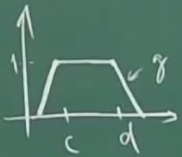
\includegraphics[width=0.3\textwidth]{images/continuous_approximation.png}
		\end{center}
	\end{enumerate}
	Теперь мы готовы рассмотреть любую $f \in L_1(\R)$ \red{не потребуется в дальнейшем?}. Заметим, что $f(x) = \lim_{N \to \infty} f(x) \cdot \chi_{[-N; N]}$. По теореме Леви снова имеем интегральный предел:
	\[
		\int_\R f(x)d\mu(x) = \lim_{N \to \infty} \int_\R f(x) \chi_{[-N; N]}d\mu(x) = \lim_{N \to \infty} \int_{[-N; N]} f(x)\chi_{[-N; N]}d\mu(x)
	\]
	Отсюда следует факт, что $\lim_{N \to \infty} \|f - f \cdot \chi_{[-N; N]}\|_{L_1(\R)} = 0$. Коль скоро носитель произведения лежит в отрезке $[-N; N]$, то интегралы по $\R$ заменяются на интегралы по $[-N; N]$. За счёт этого, мы можем воспользоваться доказанным утверждением для $L_1[-N; N]$:
	\[
		\forall N \in \N\ \forall \eps > 0\ \exists g \in T \such \|f \cdot \chi_{[-N; N]} - g\|_{L_1[-N; N]} < \eps
	\]
	Та функция $g$, которую мы находим, является гарантированно непрерывной и финитной лишь на $[-N; N]$. Чтобы получить приближающую функцию для $f$, сделаем уже известный трюк:
	\[
		g_\gamma = \System{
			&{g(x), x \in [-N; N]}
			\\
			&{0,\ x \notin [-N - \gamma; N + \gamma]}
			\\
			&{\text{линейная},\ x \in [-N - \gamma; -N] \sqcup [N; N + \gamma]}
		}
	\]
	Проверим, что $g_\gamma$ действительно приближает $f$:
	\begin{multline*}
		\|f - g_\gamma\|_{L_1(\R)} \le \|f - f \cdot \chi_{[-N; N]}\|_{L_1(\R)} + \|f \cdot \chi_{[-N; N]} - g_\gamma\|_{L_1(\R)} =
		\\
		\|f - f \cdot \chi_{[-N; N]}\|_{L_1(\R)} + \|f \cdot \chi_{[-N; N]} - g_\gamma\|_{L_1[-N; N]} + \|0 - g_\gamma\|_{L_1(\R \bs [-N; N])}
	\end{multline*}
	Величина посередине $< \eps$ в силу определения $g_\gamma$. Величину справа тоже можно сделать $< \eps$, просто выбрав достаточно малое $\gamma$. Остаётся величина слева, но она стремится к нулю при $N \to \infty$, что позволяет её тоже сделать меньше $\eps$.
\end{proof}

\begin{anote}
	При желании доказательство предыдущего утверждения можно сократить с помощью теоремы Лузина и абсолютной непрерывности интеграла Лебега. Детали остаются в качестве упражнения.
\end{anote}